\section{Blinding Magic in Delegated Quantum Computations}

\label{section:blindness}

In this section, we develop the constructions (Resources, Protocols, Simulators) necessary to blind the potential magic in a quantum computation expressed in the Clifford+MSI model. As already stated in the introduction, this is a fundamental requirement to derive classically simulable instances that could be delegated indistinguishably to the Server, and hence serve as tests that the Client can use in a verification protocol. The section is organized as follows:
\begin{itemize}
    \item In~\ref{subsection:blind:gadget}, we show how to blind the magic on a single Clifford+MSI layer, introducing the Hidden-Magic Resource~\ref{resource:blind-gate} and the Blind State Injection Protocol~\ref{protocol:blind-gate} that implements it, by applying a Pauli encryption on the input state and the injected ancilla, and compensating it later.
    \item After repeating the above protocol for each layer in the computation, what is missing to finish the computation is to perform a last Clifford layer and measurements on a state that is Pauli-encrypted. Thus, in~\ref{subsection:blind:meas}, we present the Blind Measurements Resource~\ref{resource:blind-meas} and Protocol~\ref{protocol:blind-meas} that implements it.
    \item In~\ref{subsection:blind:MB-DQC}, we compose the above protocols to implement the Magic-Blind Delegated Quantum Computing Resource~\ref{resource:mblind_DQC}. Simply composing the protocols, yielding Protocol~\ref{protocol:mblind_DQC-bf}, has a practical caveat: it implies back-and-forth communication of encrypted qubits between the Client and the Server. We show how we can safely remove this requirement and obtain the MB-DQC Protocol~\ref{protocol:mblind_DQC}, that we use throughout the rest of the paper.
    \item Lastly, in~\ref{subsection:blind:Pauli dev}, we show the powerful result that any malicious behavior from the Server—meaning applying any CPTP map instead of performing the protocol honestly—can be reduced to a convex combination of Pauli operators applied after an honest execution of the protocol, before the measurements. This arrives as a consequence of the Pauli encryption of the qubits, allowing us to perform a Pauli Twirl of any malicious behavior.
\end{itemize}
\subsection{Blinding Magic on a single layer}
\label{subsection:blind:gadget}

In the Clifford+MSI model, the only non-Clifford ingredient is the injected single-qubit state together with a simple measurement-dependent correction. This makes state injection the natural ``locus'' where a Client can hide potential magic while delegating only Clifford operations.

We therefore isolate the following elementary delegation task. The Client holds an $n$-qubit input state\footnote{Note that this differs from the typical classical inputs considered in $\BQP$ computations. This is not a problem here because in this section we do not describe a $\BQP$ computation, but quantum evolution on states of $n$ qubits.} $\rho$, chooses a public Clifford layer $\C\in\Clifford_n$, and chooses a state to inject via a label $\A$.
The goal is to implement the corresponding transformation on $\rho$ while hiding from the Server both the data $\rho$ and the choice of injection type $\A$.
This is captured by the Hidden-Magic Gate Resource~\ref{resource:blind-gate}, which we view as the circuit-model analogue of performing the Clifford layer followed by a ``blind gadget'' implementing one compiled (potentially) non-Clifford layer. The Resource supports two regimes:
\begin{enumerate}
    \item \textbf{Magic regime.} When $\Alabel=\Tlabel$, the resource performs a Magic-State Injection.
    \item \textbf{Stabilizer regime.} When $\Alabel\neq \Tlabel$ and $\rho$ is a stabilizer input, the resource returns the result of injecting state $\ket\Alabel$, including the (classically simulable) measurement outcome.
\end{enumerate}

In both regimes, the Server learns only the public information (in particular $\C$ and the system size), but gains no information about $\rho$ nor about the Client's choice $\A$. It only learns the set of possible choices $\classA=\{\Tlabel, \pm\Xlabel,  \pm\Ylabel,  \pm\Zlabel\}$.
\begin{resourcee}[h]
    \caption{Hidden-Magic Gate}
    \label{resource:blind-gate}
    \begin{algorithmic}[0]
        \State \textbf{Public Information:} $\C\in\Clifford_n$, $\classA$.
        \State \textbf{Client's Input:} $\C\in\Clifford_n, \Alabel\in\classA$, and a classical description of a quantum state $\rho$ on $n$ qubits.
        \State \textbf{Server's Input:} $\c\in\bin$, set to $0$ if honest. If $\c=1$, the Server will have the opportunity to provide more inputs.

        \Procedure{Computation by the Resource}{}
        \If{$\c=0$}
            \If{$\Alabel=\Tlabel$}
            \State Output $\T_n\circ \C[\rho]$ at the Client interface.
            \Else
            \State Resource samples $b$ with probability $\bra b
            \Tr_{1, ..., n}[\F\circ \C[\rho\otimes \rho_\Alabel]]
            \ket b$
            \State Output
            $
            (\id_n\otimes \ketbra b)
            \circ
            \F\circ \C[\rho\otimes\rho_\Alabel]
            $ at the Client interface.
            \EndIf
        \Else
            \State The Server holds a system whose reduced state in register $S$ is $\rho_S$: it sends $\rho_S$, alongside the instructions to perform a CPTP map $\mathrm D$ on $\rho$ and $\rho_S$. The Resource returns $\Tr_S[\mathrm D[\rho\otimes \rho_\Alabel\otimes \rho_S]]$ to the Client.
        \EndIf
        \EndProcedure
    \end{algorithmic}
\end{resourcee}
To implement this ideal behavior, we propose the Blind State Injection Protocol~\ref{protocol:blind-gate}, in which the goal of the Client is to have the Server perform a Clifford layer and an unknown state injection.
The way blindness works is indeed very similar to how blindness appears in UBQC \cite{BFK09universal}: states are encrypted and sent to the Server alongside the instruction to perform a rotation with a specific angle that compensates for the encryption.

To do so, the Client first encrypts all the qubits using $\QOTP$ yielding secret keys $\a, \r$, and sends them to the Server. Then she
 sends instructions to perform the Clifford layer and inject the state ($\CNOT$,
$\SWAP$, and measurement), in plain. Finally she needs to have the Server perform the correction (conditioned $\pi/2$ rotation) if $\A=\Tlabel$. This is equivalent to sending to the Server the value $\phi$ computed from the measurement outcome $b\in\bin$ and the injection type $\A\in\classA$ as
\begin{equation}
    \label{eq:blind:phi}
    \phi(\A, b) = \begin{cases}
        b\pi/2 &\text{if}\; \Alabel=\Tlabel\\
        0&\text{else}\;
    \end{cases}.
\end{equation}

Sending $\phi$ in plain would leak information about the choice of $\A$, so to avoid that, the angle needs to be \emph{blinded}: padded with a uniformly sampled angle $\theta\gets \$\Theta$, yielding a blinded angle $\delta$. The ancilla needs to be pre-rotated with the same $\theta$ so the encryption is canceled and has no impact on the final state (it only ensures the Server is blind).
The blinded angle is thus $\phi+\theta$ with a global sign that comes from the Pauli $\X$ encryption since $\Z(\alpha)\circ\X^a = \X^a\circ\Z((-1)^a\alpha)$ for any angle $\alpha$ and bit $a\in\bin$.
Hence, the logic to compute the angle $\delta$ from the plain angle $\phi\in\Theta$, secret $\theta\in\Theta$, and secret $\X$ encryption bit $a\in\bin$ is
\begin{equation}
    \label{eq:blinded angle}
    \delta(\phi, a, \theta)=(-1)^a (\phi+\theta).
\end{equation}
In practice, since the $\Z^\dagger(\delta)$ rotation is to be performed on the $n$-th qubit in the Protocol, Equation~\ref{eq:blinded angle} is used with the updated $\X$ encryption key on the $n$-th qubit, $a_n$.
Finally, Theorem~\ref{thm:blind-gate} states that the Protocol perfectly implements the ideal behavior, as established by its correctness and security proofs.

\begin{protocoll}
    \caption{Blind State Injection}
    \label{protocol:blind-gate}
    \begin{algorithmic}[1]
        \State \textbf{Public Information:} $\C\in\Clifford_n$, $\classA$.
        \State \textbf{Client's Input:} $\C\in\Clifford_n, \A\in\classA$, and a quantum state $\rho$ on $n$ qubits.

        \Procedure{Client - Encrypt and Send}{}
        \State Sample $\a, \r \gets\$\{0,1\}^n$, send $\Enc{\a}{\r}[\rho]$ to the Server.
        \State Sample $x, z \gets\$\{0,1\}$, $\theta\gets\$\Theta$, send $\Enc{x}{z}\Z(\theta)\ket{\Alabel}$ to Server register $n+1$.
        \State Set $\a \gets (\a ||x), \r\gets (\r||z)$. \Comment{Append existing keys}
        \EndProcedure

        \Procedure{Server - Clifford and State Injection}{}
        \State Apply $\C$ on the first $n$ qubits, and $\F=\SWAP_{n+1, n}\circ \CNOT_{n+1, n}$ on the total system.
        \State Measure qubit $n+1$ in the computational basis, send outcome $b$ to the Client.
        \EndProcedure

        \Procedure{Client - Computing and Blinding rotation angle}{}
        \State Compute updated keys $\a,\r \gets \F\circ\C(\a,\r)$.
        \State Decode the measurement outcome: store $b\gets b\oplus a_{n+1}$.
        \State Compute appropriate rotation angle $\phi(\Alabel, b)$ according to Equation~\ref{eq:blind:phi}.
        \State Compute blind angle $\delta(\phi, a_n, \theta)$, and send it to the Server.
        \label{protocolstep:blind angle}
        \EndProcedure

        \Procedure{Server - Blind Rotation}{}
        \State Apply rotation $\Z^\dagger(\delta)$ on the $n$-th qubit.
        \EndProcedure

        \Procedure{Client - Key update, Receive and Decrypt}{}
        \State Receive $n$ qubits from Server.
        \If{$\Alabel=\Tlabel$}
            \State Update $a_n\gets a_n\oplus b$ \Comment{Pauli correction required for MSI}
        \Else
            \State Store $b$ as classical output.
        \EndIf
        \State Truncate $\a, \r$ to the first $n$ bits, and apply $\Dec{\a}{\r}$ on the received qubits.
        \EndProcedure

    \end{algorithmic}
\end{protocoll}

\begin{theorem}
\label{thm:blind-gate}
The Blind State Injection Protocol~\ref{protocol:blind-gate} perfectly constructs the Hidden-Magic Gate Resource~\ref{resource:blind-gate}.
\end{theorem}

\begin{proof}[Proof of correctness (sketch, formal in~\ref{appendix: correctness of blind-gate})]
    The Protocol consists of applying the Clifford circuit, performing a measurement, and the appropriate correction (rotation, and Pauli in the magic regime) on a state that is initially encrypted by a $\QOTP$ by the Client, which is a Pauli encryption. Since all the operations that are performed are Clifford, the evolution of the pad can be tracked efficiently by the Client so the state and measurement outcome can be correctly un-padded. Lastly, the $\Z^\dagger(\delta)$ rotation is performed on the $n$-th qubit; by Equation~\ref{eq:blinded angle}, this exactly implements the required correction while compensating for both the Pauli $\X$ encryption and the ancilla pre-rotation. The presence of encryption and the fact that the ancilla is pre-rotated are therefore fully accounted for in Equation~\ref{eq:blinded angle}.
\end{proof}

\begin{proof}[Security proof]
  For the security proof, we are interested in proving the existence of a Simulator such that any malicious behavior by the Server in the Real World in Protocol~\ref{protocol:blind-gate} can be reproduced by the Simulator interacting with Resource~\ref{resource:blind-gate} in the Ideal World. Formally, both scenarios must be indistinguishable from the point of view of an unbounded Distinguisher that controls both the Client inputs and the Server deviation.
    This means that the \textit{transcript}---the total quantum state perceived by the distinguisher in one scenario for a chosen input and choice of malicious behavior---generated in both scenarios must be statistically indistinguishable.

  Figure~\ref{subfigure:secproof:initial} captures the interactions in the Real World. Playing both the Client and the Server roles, the Distinguisher chooses the input (quantum state and state label) and a cheating behavior that respects the interfaces of the Protocol, meaning that it sends a bit $b$ to the Client.
      \begin{figure}[h]
            \centering
            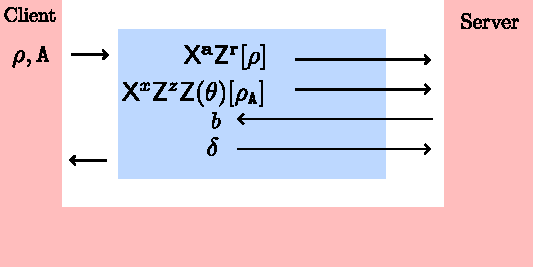
\includegraphics{figures/secproof-initial.pdf}
            \caption{Representation of the interactions between a Client and a potentially malicious Server in Protocol~\ref{protocol:blind-gate}, using the color code of Figure~\ref{fig:prelims:AC}.
            The Client protocol blinds the input state, prepares and blinds the ancilla, and sends the resulting states to the Server. When receiving a bit $b$ from the Server, the blind angle $\delta$ is computed and sent to the Server. Finally, the Client receives $n$ qubits from the Server.
            }
            \label{subfigure:secproof:initial}
    \end{figure}

  To prove the existence of a Simulator that can be plugged in Resource~\ref{resource:blind-gate} to reproduce this behavior, we do the following.
   We reproduce the steps of \cite{DFPR14composable}, and present Reduction~\ref{protocol:blind-gate-reduction}: it is an EPR reduction of Protocol~\ref{protocol:blind-gate} (using the terminology introduced in the preliminaries), in which the Client uses the fact that measurements are delayed to choose and send a uniformly distributed rotation angle $\delta$ and compute $\theta$ simply by inverting Equation~\ref{eq:blinded angle}:
  \begin{equation}
    \label{eq:blinded angle inverted}
    \theta = (-1)^{a}\delta - \phi.
  \end{equation}
  Then, we show that this Reduction can instead be performed by a Simulator plugged in the Resource.
  On Figure~\ref{subfigure:secproof:epr}, we represent the first part of the reduction: replacing $\QOTP$ by EPR-encryption in the Client part of the Protocol. The transcript (\textit{i.e} the overall quantum state perceived by the Distinguisher: the $n$ qubit state, the ancilla qubit, and the rotation) generated in this version is clearly identical to the one generated by the initial protocol, by correctness of this EPR-realization of the $\QOTP$ (see \cite{SP00simple} and preliminaries). At this stage, when measurement outcomes are $\a, \r$, $x, z$, according to the notations of Figure~\ref{subfigure:secproof:epr}, the Server holds the state $\Enc{\a}{\r}[\rho]\otimes \Enc{x}{z}\circ\Z(\theta)[\rho_\Alabel]$, identical to what it holds in Protocol~\ref{protocol:blind-gate}
  for the same key bits obtained by uniform sampling.
      \begin{figure}[h]
            \centering
            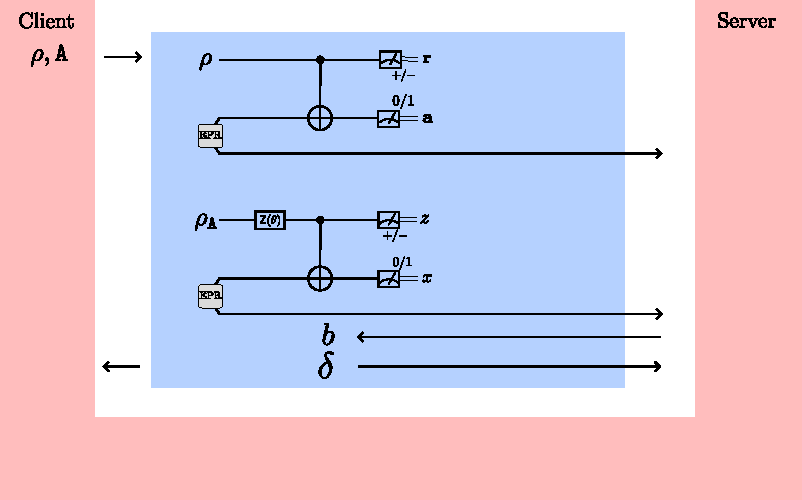
\includegraphics{figures/secproof-EPR.pdf}
            \caption{Same as Figure~\ref{subfigure:secproof:initial}, but the Client part of the Protocol used EPR-encryption to perform the $\QOTP$ on the $n$-qubit state $\rho$, and on the single-qubit, ancilla pre-rotated with $\Z(\theta)$.
            }
            \label{subfigure:secproof:epr}
    \end{figure}

    Then, to reach Reduction~\ref{protocol:blind-gate-reduction}, we use a delayed-measurement trick to show that instead of choosing $\theta$ at random and computing $\delta$ from it using Equation~\ref{eq:blinded angle}, the Client can choose $\delta$ at random and compute $\theta$ from it using Equation~\ref{eq:blinded angle inverted}. Indeed, on Figure~\ref{subfigure:secproof:epr}, the $\Z(\theta)$ commutes with the control: it can thus be delayed and performed right before the Hadamard-basis measurement that yields outcome $z$, which is then stored as $r_{n+1}$.
    Now we make the following two observations, captured in Lemma~\ref{lemma:blind-gate:key dependency}.
    The first one is that $a'_n$ (the bit used in the rotation angle logic) does not depend on $r_{n+1}$. The other one is that $a'_{n+1}$ (the bit used to decode the measurement outcome) neither.
    Therefore, since $r_{n+1}$ is not needed to compute $a'_n$ nor $a'_{n+1}$, this measurement can be delayed to after the interaction with the Server.

    \begin{lemma}
        \label{lemma:blind-gate:key dependency}
        Let there be a $n+1$-qubit system, $\C\in\Clifford_n$ and $\F=\SWAP_{n+1,n}\circ\CNOT_{n+1,n}$. Let $\a, \r\in\bin^{n+1}$ Pauli encryption keys and $\a', \r'=\F\circ \C(\a, \r)$. Then, neither $a'_n$ nor $a'_{n+1}$ depend on $r_{n+1}$.
    \end{lemma}
    \begin{proof}
        This can be proven just by analyzing how the $\Z$-encryption on the $n+1$-th qubit commutes through $\F\circ \C$. Since $\C$ acts on the first $n$ qubits, it commutes trivially. Then, through $\F$, it commutes through the control of the $\CNOT$ and ends as a $\Z$ encryption on the $n$-th qubit after the $\SWAP$. Hence, we conclude that $r_{n+1}$ does not influence $a'_{n}$ nor $a'_{n+1}$.
    \end{proof}

    Thus, in Reduction~\ref{protocol:blind-gate-reduction}, the Client first chooses $\delta$ uniformly at random, and computes $\theta$ from Equation~\ref{eq:blinded angle inverted}, without changing the distribution of the overall state.
    Finally, the Client performs the delayed $\Z(\theta)$ rotation and the Hadamard basis measurement to obtain $r_{n+1}$ and re-compute the updated keys to decrypt the qubits identically as in the original version.
    This is depicted on Figure~\ref{secproof:delayedrot}: for the same choice of inputs and malicious behavior, this interaction produces the same transcript as the initial Protocol in Figure~\ref{subfigure:secproof:initial}.
            \begin{figure}[h]
            \centering
            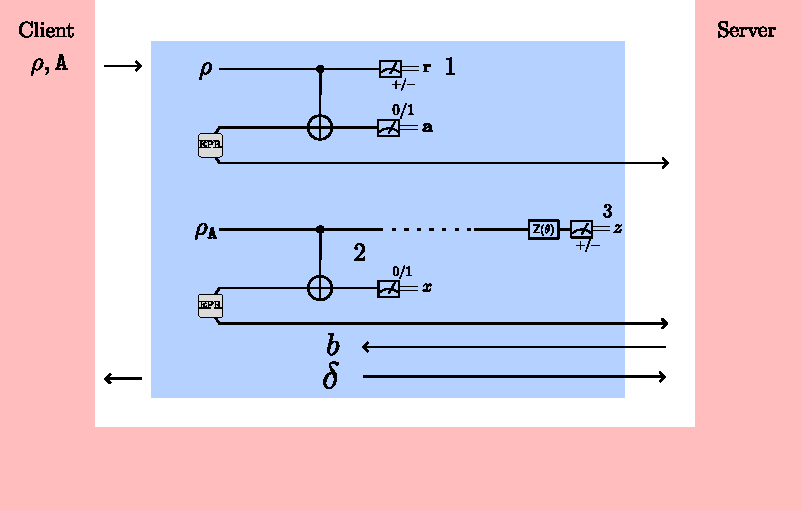
\includegraphics{figures/secproof-delayed.pdf}
            \caption{Illustration of the interactions in Reduction~\ref{protocol:blind-gate-reduction}, using the same color code as in Figure~\ref{subfigure:secproof:initial}. Here, the difference with Figure~\ref{subfigure:secproof:epr} is that $\delta$ is sampled uniformly and sent to the Server before the $n+1$-th encryption bit $z$ (equivalently $r_{n+1}$) is obtained, and $\theta$ is computed from $\delta$ according to Equation~\ref{eq:blinded angle inverted}.}
            \label{secproof:delayedrot}
    \end{figure}

    Finally, we introduce Simulator~\ref{simulator:blind-gate}: it deals with the Server interactions the same way as the Client in Reduction~\ref{protocol:blind-gate-reduction}, and lets the input-dependent operations be performed by Resource~\ref{resource:blind-gate}, according to its description (in the malicious scenario $c=1$, the Resource receives a quantum state and a CPTP map).
    The interaction generates the same transcript, since the same operations are being performed, just by different entities. In Figure~\ref{secproof:simulator}, the same operations as in Figure~\ref{secproof:delayedrot} are carried out, but some by the Simulator---preparing EPR pairs and sending random $\delta$---while the rest are carried out by a CPTP map that the Simulator asks the Resource to perform, according to the description of Resource~\ref{resource:blind-gate}.
    Therefore, for a given Client input and Server cheating behavior, the same transformation as in the initial protocol is being implemented, but by the Simulator plugged into the Ideal Resource, and hence the two worlds are indistinguishable from the point of view of the Distinguisher, which concludes the proof.

    \begin{figure}[h]
            \centering
            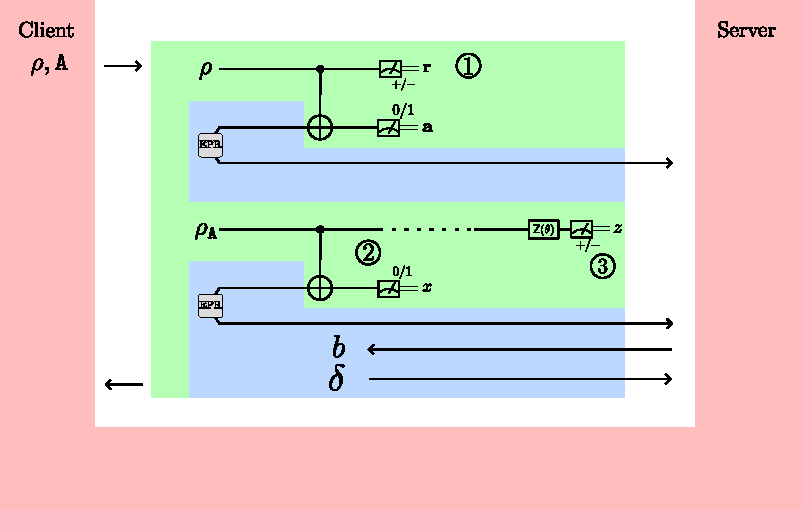
\includegraphics{figures/secproof-simulator.pdf}
            \caption{Same interaction as Figure~\ref{secproof:delayedrot}, but now the blue box represents \textbf{Simulator}~\ref{simulator:blind-gate}, and the green box represents the CPTP map performed by the Ideal Resource: step $1$ is the encryption of $\rho$, step $2$ is the EPR-encryption of $\rho_\A$ part 1, and step $3$ is part 2. Compared to Figure~\ref{subfigure:secproof:initial}, the execution of Protocol~\ref{protocol:blind-gate} has been replaced by Simulator~\ref{simulator:blind-gate} plugged into Resource~\ref{resource:blind-gate} with the required instructions to reproduce the deviation chosen by the Server interface of the Distinguisher. Since the transcript generated by the interactions in Figure~\ref{subfigure:secproof:initial} and the current figure are indistinguishable (given a choice of inputs/deviation from the Distinguisher), the two scenarios are indistinguishable and therefore the composable security is proven.}
            \label{secproof:simulator}
    \end{figure}

\begin{reduction}
    \caption{Blind State Injection, EPR-Client, malicious Server (reduction)}
    \label{protocol:blind-gate-reduction}
    \begin{algorithmic}[1]
        \State $\triangleright$ \textsc{Client - } Prepare $n$ EPR-pairs and send half of each pair to the Server.
        \Procedure{Client - EPR-encryption of $\rho$}{}
        \For{$1\leq i\leq n$}
            \State Apply $\CNOT$ on $i$-th qubit of $\rho$ (as control) and its $i$-th EPR-half (as target).
            \State Measure the $i$-th EPR half in computational basis, label the outcome $a_i$.
            \State Measure $i$-th qubit of $\rho$ in the Hadamard basis, label the outcome $r_i$.
        \EndFor
        \State Write the resulting $n$-bit strings $\a, \r$.
        \EndProcedure

        \State$\triangleright$ \textsc{Client - } Prepare an EPR-pair and send half to the Server.
        \Procedure{Client - EPR-encryption of ancilla, part 1}{}
        \State Prepare $\rho_\A=\ketbra{\A}$.
        \State Apply $\CNOT$ on $\rho_\A$ (as control) and the EPR-half (as target).
        \State Measure the EPR-half in the computational basis, and label the outcome $x$.
        \State Set $\a' \gets (\a ||x), \r'\gets (\r||0)$, as $z$ is obtained only in part 2.
        \EndProcedure

        \State$\triangleright$ \textsc{Client - } receives bit $b$ from Malicious Server.

        \Procedure{Client - Computing and Blinding rotation angle}{}
        \State Compute $\a', \r' \gets \F\circ \C(\a', \r')$. Note that $z$ does not affect $a'_{n+1}$ nor $a'_n$, which are the only ones we need for this step.
        \State Decode the measurement outcome: receive $b$, store $b\gets b\oplus a'_{n+1}$.
        \State Compute appropriate measurement angle $\phi(\A, b)$.
        \EndProcedure
        \State $\triangleright$\textsc{Client - } Sample random rotation angle uniformly. $\delta\gets\$\Theta$ and send it to the Server.

        \Procedure{Malicious Server - Blind Rotation}{}
        \EndProcedure

        \Procedure{Client - EPR-encryption of ancilla, part 2}{}
        \State Compute appropriate pre-rotation angle $\theta(\phi, a'_n, \delta)=(-1)^{a'_n}\delta - \phi$.
        \State Apply $\Z(\theta)$ on the ancillary qubit, measure in the Hadamard basis, label the outcome $z$.
        \State Set $\a \gets (\a ||x), \r\gets (\r||z)$ and re-compute key-update: $\a, \r = \F\circ \C(\a, \r)$.
        \EndProcedure

        \Procedure{Client - Key update, Receive and Decrypt}{id. Protocol~\ref{protocol:blind-gate}}
        \EndProcedure

    \end{algorithmic}
\end{reduction}

\begin{simulatorr}
    \caption{Blind State Injection}
    \label{simulator:blind-gate}
    \begin{algorithmic}[1]
        \Procedure{Simulator - Emulates Client interaction with Server}{}
        \State Prepare $n+1$ EPR Pairs, and send each half to the Server.
        \State Receive bit $b$ from the Server.
        \State Sample $\delta \gets \$\Theta$ and send it to the Server.
        \EndProcedure

        \Procedure{Simulator - Make Resource reproduce the Server behavior}{}
        \State Send the remaining $n+1$ EPR halves, $b$, and $\delta$ to Ideal Resource
        \State Send the below instructions as a CPTP map to the Resource to perform.
        \EndProcedure
        \Procedure{CPTP map sent to the Resource}{$\A, \rho$ from Client ; $n+1$ EPR-halves, $\delta, b$ from Simulator}
        \State EPR-encryption of $\rho$
        \State EPR-encryption of $\rho_\A$, part 1
        \State Compute rotation angle
        \State EPR-encryption of ancilla, part 2
        \State Key update, Receive and Decrypt
        \EndProcedure

    \end{algorithmic}
\end{simulatorr}
 \end{proof}
\subsection{Blind measurements}
\label{subsection:blind:meas}
In this section, we introduce the ideal functionality allowing a Client to delegate the execution of a Clifford circuit on $n$ qubits followed by a measurement of the $n$ qubits in the computational basis, with the security property that the Server performs these steps blindly on the data sent by the Client. Indeed, Resource~\ref{resource:blind-meas} captures this security property: the Server learns the intended Clifford circuit $\C$ and the size of the system, but not $\rho$ the $n$-qubit input of the Client, while the Client receives $\z$ sampled by the $\Z$-basis measurement distribution of the state $\C[\rho]$.
\begin{resourcee}
    \caption{Blind measurements}
    \label{resource:blind-meas}
    \begin{algorithmic}[1]
        \State \textbf{Public Information:} $n, \C$ and basis of measurements (computational basis).
        \State \textbf{Client's Input:} $n$-qubit quantum state $\rho$, Clifford circuit
        \State \textbf{Server's Input:} $\c\in\bin$, set to $0$ if honest. If $\c=1$, the Server will have the opportunity to provide more inputs.
        \Procedure{Computation by the Resource}{}
        \If{$\c=0$}
            \State Sample $\z$ with probability $\bra \z \C[\rho]\ket \z$
            \State Output $ \ketbra \z \circ \C[\rho]$
        \Else
            \State The Server holds a system whose reduced state in register $S$ is $\rho_S$: it sends $\rho_S$, alongside the instructions to perform a CPTP map $\mathrm D$ on $\rho$ and $\rho_S$. The Resource returns $\Tr_S[\mathrm D[\rho\otimes \rho_S]]$ to the Client.
        \EndIf
        \EndProcedure
    \end{algorithmic}
\end{resourcee}
We introduce Protocol~\ref{protocol:blind-meas} to implement this resource, which makes the simple use of a Quantum One-Time Pad applied on $\rho$ before being sent to the Server, and a decoding of the measurement outcome by a Pauli operator resulting of conjugating the initial Pauli (used for encryption) by the Clifford circuit performed by the Server.

\begin{protocoll}
    \caption{Blind measurements}
    \label{protocol:blind-meas}
    \begin{algorithmic}[1]
        \State \textbf{Public Information:} $n, \C$ and basis of measurements (computational basis).
        \State \textbf{Client's Input:} $n$-qubit quantum state $\rho$, Clifford circuit $\C\in\Clifford_n$.

        \Procedure{Client - Encrypt and Send}{}
        \State Sample $\a, \r\gets \bin^{n}$ and send $\Enc{\a}{\r}[\rho]$ to Server
        \EndProcedure

        \Procedure{Server - Clifford circuit and measurements}{}
        \State Perform $\C$ on the received qubits.
        \State Measure all the qubits in the computational basis, getting the $n$-bit outcomes $\z$
        \EndProcedure

        \Procedure{Client - Decode measurement outcomes}{}
        \State Client updates keys as $\a, \r\gets \C(\a, \r)$
        \State Store $\z\oplus \a$ as output of the protocol.
        \EndProcedure
    \end{algorithmic}
\end{protocoll}

\begin{theorem}
    \label{thm:blind-meas}
    The Blind Measurements Protocol~\ref{protocol:blind-meas} perfectly constructs Resource~\ref{resource:blind-meas}
    in the Abstract Cryptography framework.
    \end{theorem}

\begin{proof}[Proof of correctness]
    When both parties are honest, the Server receives $\Enc{\a}{\r}[\rho]$, applies $\C$, performs a computational-basis measurement of all qubits, and sends the measurement outcomes in an $n$-bit string $\z$ to the Client. The Client computes the conjugation of the initial encryption by the Clifford circuit, which gives $\a', \r'=\C(\a, \r)$, and stores $\z\oplus\a'$ as the output of the protocol. Formally, the output of the Client can thus be written
    \begin{align}
        \rho_{out, \z\oplus\a'} &=
        \ketbra{\z\oplus\a'}{\z}
        \circ
        \C
        \circ \Enc{\a}{\r}[\rho]
        \\
        &=
        \ketbra{\z\oplus\a'}{\z}
        \circ
        \Enc{\a'}{\r'}
        \circ
        \C
        [\rho].
    \end{align}
    With a change of variables $\z'= \z\oplus \a'$, then $\z$ becomes $\z'\oplus \a'$, and the expression becomes
    \begin{align}
        \rho_{out, \z'}
        &=
        \ketbra{\z'}{\z'\oplus \a'}
        \circ
        \Enc{\a'}{\r'}
        \circ
        \C
        [\rho]
        \\
        &=
        \ketbra{\z'}{\z'}
        \circ
        \X^{\a'}
        \circ
        \Enc{\a'}{\r'}
        \circ
        \C
        [\rho]
        \\
        &=
        \ketbra{\z'}{\z'}
        \circ
        \Dec{\a'}{\r'}
        \circ
        \Enc{\a'}{\r'}
        \circ
        \C
        [\rho]
        \\
        &=
        \ketbra{\z'}{\z'}
        \circ
        \C
        [\rho].
    \end{align}
    Thus, the output of the protocol is a bitstring $\z$ that follows the distribution $p(\z)=\bra\z\C[\rho]\ket\z$, identically to the output of Resource~\ref{resource:blind-meas}.
\end{proof}

\begin{proof}[Security proof (sketch, formal in~\ref{section:blindmeas-secproof-formal})]
     Here, we aim to present a Simulator that uses only the public information and interacts with Resource~\ref{resource:blind-meas} in a way that makes the Real World indistinguishable from the Ideal World for an unbounded distinguisher.
     To do so, we start by carrying out an EPR reduction of Protocol~\ref{protocol:blind-meas}: performing the Pauli encryption using EPR pairs and Bell measurements. Doing so clearly results in the same transformation from the Distinguisher's point of view. Then, we show that the same transformation can be reached by Simulator~\ref{simulator:blind-meas}, which uses only the public information and interacts with Resource~\ref{resource:blind-meas}. The equivalence is straightforward, as Simulator~\ref{simulator:blind-meas} performs the steps of the EPR reduction that do not require the input state, while instructing the Resource to do the rest.
     This concludes the proof, as in the presence of a malicious Server, Protocol~\ref{protocol:blind-meas} is indistinguishable from Simulator~\ref{simulator:blind-meas} plugged in Resource~\ref{resource:blind-meas} from an unbounded Distinguisher.

\begin{simulatorr}
    \caption{Blind Measurements}
    \label{simulator:blind-meas}
    \begin{algorithmic}[1]
        \State \textbf{Simulator Inputs:} $n, \C$ and basis of measurements (computational basis).
        \Procedure{Simulator - Emulates Client interaction with Server}{}
        \State Prepare $n$ EPR Pairs, and send each half to the Server.
        \State Receive $n$-bit string $\z$ from the Server.
        \EndProcedure

        \Procedure{Simulator - Make Resource reproduce the Server behavior}{}
        \State Send the remaining $n$ EPR halves and $\z$ to Ideal Resource.
        \State Send the below instructions as a CPTP map to the Resource to perform.
        \EndProcedure

        \Procedure{CPTP map sent to the Resource}{$\C, \rho$ from Client; $n$ EPR-halves, $\z$ from Simulator}
        \State EPR-encryption of $\rho$
        \State Decode measurement outcomes
        \EndProcedure
    \end{algorithmic}
\end{simulatorr} \end{proof}

\subsection{Magic-Blind Delegated Quantum Computations}
\label{subsection:blind:MB-DQC}
We now complete our goal of providing magic-blindness by composing the previously introduced protocols: we show how to hide the magic of an entire delegated computation $$C \;=\; \C_{t+1}\circ \T_n \circ \C_t \circ \cdots \circ \T_n \circ \C_1$$ followed by computational basis measurements where $\C_i\in\Clifford_n$ are Clifford layers and each $\T_n$ is implemented by a state-injection gadget acting on the $n$-th wire.
\subsubsection{Ideal functionality and induced computation class}
The blindness requirement is captured by the Magic-Blind Delegated Quantum Computation Resource~\ref{resource:mblind_DQC}.
\begin{resourcee}
    \caption{Magic-Blind DQC}
    \label{resource:mblind_DQC}
    \begin{algorithmic}[0]
        \State \textbf{Public Information:} $n, t, \C_1...\C_{t+1}$ and basis of measurements (computational basis).
        \State \textbf{Client's Inputs:} classical input $\x\in\bin^n$, $\C_1...\C_{t+1}\in\Clifford_n$ and $\{\A_i\in\classA\}_{i\leq t}$.
        \State \textbf{Server's Input:} $\c\in\bin$, set to $0$ if honest. If $\c=1$, the Server will have the opportunity to provide more inputs.

        \Procedure{re-naming}{}
        \State  $\star=1$ if $\A_i=\Tlabel$ for all $i$, $\star=0$ if $\A_i\neq \Tlabel$ for all $i$.
        \State  $\G=\C_{t+1}
        \circ \F_t\circ \C_t
        \circ \cdots
        \circ \F_1\circ \C_1$
        ,  $\rho_\x=\ketbra \x$
        ,  $\rho_\A=\bigotimes_{i=1}^t\rho_{\A_i}$
        \EndProcedure

        \Procedure{Computation by the Resource}{}
        \If{$\c=0$}
        \If{$\star$}
        \State Sample $\b$ with probability $\bra \b \C_{t+1}
        \circ
        \T_n\circ \C_t \circ \cdots \T_n\circ \C_1[\rho_\x]\ket \b$
        \State Output $
       \ketbra\b
        \circ
        \C_{t+1}
        \circ
        \T_n\circ \C_t \circ \cdots \T_n\circ \C_1[\rho_\x]
        $.
        \Else{}
        \State Sample $\b$ with probability $\bra \b \G[\rho_\x\otimes \rho_\A] \ket \b$
        \State Output $
        \ketbra\b
        \circ
        \G[\rho_\x\otimes \rho_\A]
        $.
        \EndIf
        \Else
        \State The Server holds a system whose reduced state in register $S$ is $\rho_S$: it sends $\rho_S$, alongside the instructions to perform a CPTP map $\mathrm D$ on the entire system. The Resource returns $\Tr_S[\mathrm D[\rho_\x\otimes \rho_\Alabel\otimes \rho_S]]$ to the Client.
        \EndIf
        \EndProcedure
    \end{algorithmic}
\end{resourcee}
The Client provides an $n$-bit input $\x$ and, for each injection step $i\leq t$, a choice $\A_i\in\classA$ specifying which single-qubit state is injected.
The public input to the resource consists of the Clifford structure $\C_1,\ldots,\C_{t+1}$, which is explicitly leaked to the Server. On the other hand, the inputs of the Client (choice of inputs and injections) are kept hidden from the Server, which constitutes the magic-blindness functionality.
The resource supports two operational modes, captured by $\star$ in Resource~\ref{resource:mblind_DQC}:
\begin{itemize}
    \item \textbf{Computation mode}, where $\A_i=\Tlabel$ for all $i\leq t$.
    In this case, the resource performs the target non-Clifford computation $C$ on input $\rho$ and returns the resulting measurement outcomes to the Client.
    \item \textbf{Magic-free mode}, where $\A_i\neq\Tlabel$ for all $i\leq t$.
    Here, all injections are stabilizer injections and the resulting transformation on the enlarged $n+t$ qubit system is Clifford. The outcomes correspond to a classically simulable computation—cf. Section~\ref{subsection:prelims:QC}, since input states are all stabilizers, transformation is Clifford, and measurements are Pauli—and serve only for testing.
\end{itemize}

In the magic-free mode, it is convenient to make the induced Clifford structure explicit. Writing $\F_i=\SWAP_{n+i,n}\circ\CNOT_{n+i,n}$ for the Clifford circuit implementing the $i$-th injection gadget, the overall transformation applied to the joint input $\rho_\x\otimes\rho_\A$ (where $\rho_\A=\bigotimes_{i=1}^t\rho_{\A_i}$) is the Clifford circuit
\begin{equation}
    \label{eq:blindness:G}
\G \;=\; \C_{t+1}\circ \F_t \circ \C_t \circ \cdots \circ \F_1 \circ \C_1,
\end{equation}
also depicted at Figure~\ref{fig:blindness:G}.
A final layer of computational-basis measurements is then applied to the remaining unmeasured qubits. Crucially, the Server observes the same sequence of Clifford operations in both modes.

\begin{figure}[h]
    \centering
    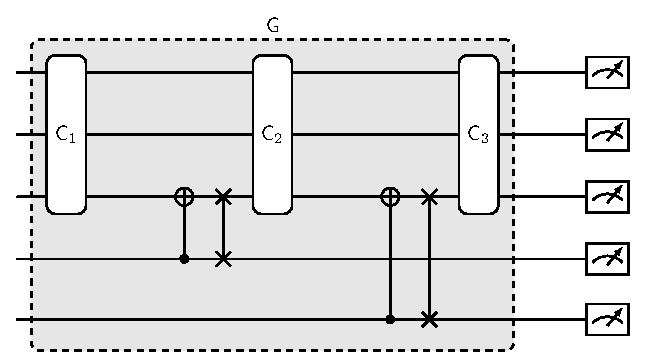
\includegraphics[]{tikz-figures/magic-free/test.pdf}
    \caption{The Clifford transformation $\G$ that is implemented on $n+t$ qubits in the magic-free mode. Rotation angles are replaced by $0$, and no Pauli correction is being made.}
    \label{fig:blindness:G}
\end{figure}

\paragraph{Class of indistinguishable computations.}
By construction, Resource~\ref{resource:mblind_DQC} induces a natural \textit{class of computations that are indistinguishable to the Server under magic-blind delegation}, that we write $\class$.
All computations in this class share the same public Clifford structure $\C_1,\ldots,\C_{t+1}$, but may differ in their injected single-qubit states and in the associated measurement-angle logic.
In particular, $\class$ contains:
\begin{itemize}
    \item the \emph{target computation}, obtained by injecting magic states
    $\rho_\A=\bigotimes_{i\leq t}\T[\ketbra{+}]$ and using the measurement-dependent correction
    angles $\phi_i=b_i\pi/2$;
    \item a family of \emph{test computations}, obtained by injecting stabilizer states
    $\rho_{\A_i}\in\{\pm\ket \Xlabel,\pm\ket \Ylabel,\pm\ket \Zlabel\}$, for which the circuit does not need adaptivity and can use fixed angles
    (here set to $\phi_i=0$).
\end{itemize}

Without surprise, we propose the Magic-Blind Delegated Quantum Computation Protocol~\ref{protocol:mblind_DQC-bf}, a sequential composition of $t$ instances of the Blind State Injection Protocol~\ref{protocol:blind-gate}, adapting the injected ancilla, Clifford circuit, and ancilla index to the layer; then followed by the Blind Measurements Protocol~\ref{protocol:blind-meas}. As for the ideal behavior, it supports two modes: either $\A_i=\Tlabel$ for all $i$ (computation), or for no $i$ (magic-free). This is captured by a $\star$ in Protocol~\ref{protocol:mblind_DQC-bf}.
\begin{protocoll}
    \caption{Magic-Blind Delegated Quantum Computation (MB-DQC)}
    \label{protocol:mblind_DQC-bf}
    \begin{algorithmic}[1]
        \State \textbf{Public Information:} $n, t, \C_1...\C_{t+1}$ and basis of measurements (computational basis).
        \State \textbf{Client's Inputs:} classical input $\x\in\bin^n$, $\C_1...\C_{t+1}$ and $\A_i\in\classA$ for $i\leq t$.

        \State Client sets her computation register to $\rho_\x = \ketbra \x$.
        \Procedure{Clifford and Blind Gadget layers}{}
            \For{$i\leq t$}
                \State Client and Server perform Protocol~\ref{protocol:blind-gate} with the Client's computation register on inputs $\C_i, \A_i$ and ancilla register $n+i$ instead of $n+1$.
                \State
                Client sets the received $n$
                 qubits in her computation register, and if $\A_i\neq\Tlabel$ sets the received classical bit to $b_i$.
            \EndFor
        \EndProcedure

        \Procedure{Clifford and Blind measurements}{}
            \State Client and Server perform Protocol~\ref{protocol:blind-meas} on Clifford $\C_{t+1}$ and the Client's computation register.
            \State Output: Client receives $n$-bit string $\x$.
        \EndProcedure

        \Procedure{Output}{}
        \If{$\star$}
        \State \textbf{Output:} set $\b\gets \x$ and output $\b$.
    \Else
        \State \textbf{Output:} set $\b\gets \x\ \|\ b_1\ \|\ \cdots\ \|\ b_t$ and output $\b$.
    \EndIf
        \EndProcedure
    \end{algorithmic}
\end{protocoll}

\begin{theorem}
    \label{thm:mblind_DQC}
    The Magic-Blind Delegated Quantum Computation Protocol~\ref{protocol:mblind_DQC-bf} perfectly constructs Resource~\ref{resource:mblind_DQC}
    in the Abstract Cryptography framework.
    \end{theorem}
\begin{proof}
    This can be proven straightforwardly using the composability of the protocols presented before, since Resource ${\ref{resource:mblind_DQC}}$ on inputs $\C_1, ..., \C_{t+1}$, and $\A_1, ..., \A_t$ can be realized by using Resource~\ref{resource:blind-gate} on $\C_1, \A_1$ and index $1$, then again on $\C_2, \A_2$, and index $2$, and so on, and finally Resource~\ref{resource:blind-meas} with input $\C_{t+1}$.
      Formally, using the notations of the AC framework and denoting by $\Protocol_{\ref{protocol:blind-gate}}$ the converter of the Blind State Injection Protocol~\ref{protocol:blind-gate}, and by $\Protocol_{\ref{protocol:blind-meas}}$ the converter of the Blind Measurements Protocol~\ref{protocol:blind-meas}, we have:
      \begin{align}
          \Resource_{\ref{resource:mblind_DQC}}(\C_1, ..., \C_{t+1};\A_1, ..., \A_t)
          &=
          \Resource_{\ref{resource:blind-meas}}(\C_{t+1})
          \circ
          \Resource_{\ref{resource:blind-gate}}(\C_t; \A_t; t)
          \circ
          \cdots
          \circ
          \Resource_{\ref{resource:blind-gate}}(\C_1; \A_1; 1)
          \\
          &=
          \left( \Protocol_{\ref{protocol:blind-meas}}(\C_{t+1})
          \circ
          \Protocol_{\ref{protocol:blind-gate}}(\C_t; \A_t; t)
          \circ
          \cdots
          \circ
          \Protocol_{\ref{protocol:blind-gate}}(\C_1; \A_1; 1) \right)\qchannel
          \\
          &=
          \Protocol_{\ref{protocol:mblind_DQC-bf}}(\C_1, ..., \C_{t+1};\A_1, ..., \A_t) \qchannel.
      \end{align}
  \end{proof}

\subsubsection{Removing the back-and-forth communication between Client and Server}
Protocol~\ref{protocol:mblind_DQC-bf} has a practical caveat. It uses a two-way quantum communication channel since it requires the Client, for consecutive calls to Protocol~\ref{protocol:blind-gate}, to receive $n$ qubits, decrypt them, encrypt them again, and re-send them---this is also the case for the last call between Protocol~\ref{protocol:blind-gate} and Protocol~\ref{protocol:blind-meas}. In this section, we show that this "back-and-forth" communication can be removed. The first forward (encrypted) quantum communication is still required. Then, instead of receiving, decrypting, re-encrypting, and re-sending qubits, the Client can simply instruct the Server to keep the qubits while treating the decryption keys as new encryption keys kept hidden from the Server. Doing so yields Protocol~\ref{protocol:mblind_DQC}. Indeed, we replace the textbook execution of Protocols~\ref{protocol:blind-gate} and~\ref{protocol:blind-meas} by equivalent procedures in which the Client neither sends freshly encrypted qubits nor receives qubits to decrypt, since the Server keeps the qubits.
\begin{protocoll}
\caption{MB-DQC (without Back-And-Forth)}
\label{protocol:mblind_DQC}
\begin{algorithmic}[1]
\State \textbf{Public:} $\C_1,\ldots,\C_{t+1}\in\Clifford_n$
\State \textbf{Client input:}  $\x\in\bin^n$, $\A_i\in\classA$ for $i\le t$
\State \textbf{Notation:} $\star$ if $\A_i=\Tlabel$ for all $i\leq t$. Steps with "\textbf{C}" are done by the Client, "\textbf{S}" by the Server.

\Procedure{Blind-State Injection}{$i,\C,\A;\ (\a,\r)$}
  \State \textbf{C:} sample $x,z\gets\$\{0,1\}$, $\theta\gets\$\Theta$.

  \State \textbf{C:} prepare $\Enc{x}{z}\Z(\theta)\ket{\Apattern}$ and send to Server register $n+i$.
  \State \textbf{C:} set $(\a,\r) \gets(\a\|x,\ \r\|z)$.
  \State \textbf{S:} apply $\C$ and then $\F_i := \SWAP_{n+i,n}\circ\CNOT_{n+i,n}$.
  \State \textbf{S:} measure qubit $n+i$ in computational basis; send outcome $b_i$.
  \State \textbf{C:} update keys $(\a,\r)\gets (\F_i\circ \C)(\a,\r)$.
  \State \textbf{C:} decode $b_i \gets b_i \oplus a_{n+i}$.
  \State \textbf{C:} compute appropriate rotation angle $\phi(\A_i, b_i)$.
  \State \textbf{C:} compute blind angle $\delta(\phi, a_n, \theta)$.
  \State \textbf{S:} apply $\Z^\dagger(\delta)$ on qubit $n$.
  \If{$\A=\Tlabel$}
    \State \textbf{C:} $a_n \gets a_n \oplus b_i$ \Comment{Pauli correction for MSI}
  \EndIf
  \State \textbf{Output:} updated $(\a,\r)$ and (if $\A\neq\Tlabel$) the classical bit $b_i$.
\EndProcedure

\Procedure{Blind Measurements}{$\C;\ (\a,\r)$}
  \State \textbf{S:} apply $\C$ and measure all qubits in the computational basis, obtaining $\z$.
  \State \textbf{C:} update keys $(\a,\r)\gets \C(\a,\r)$ and output $\z\oplus \a$.
\EndProcedure

\Statex
\Procedure{Computation}{}
  \State \textbf{C:} sample $(\a,\r)\gets\$\{0,1\}^{n}\times\{0,1\}^{n}$ and send $\Enc{\a}{\r}[\rho]$.
  \For{$i=1, ..., t$}
    \State run \textsc{Blind-State Injection}$(i,\C_i,\A_i;\ (\a,\r))$;
          store classical bit as $b_i$ if $\A_i\neq\Tlabel$.
  \EndFor
  \State Run \textsc{Blind Measurements}$(\C_{t+1};\ (\a,\r))$, output $\z$.
  \If{$\star$}
    \State \textbf{Output:} set $\b\gets \z$ and output $\b$.
  \Else
    \State \textbf{Output:} set $\b\gets \z\ \|\ b_1\ \|\ \cdots\ \|\ b_t$ and output $\b$.
  \EndIf
\EndProcedure
\end{algorithmic}
\end{protocoll}

\begin{theorem}
    \label{thm:mblind_DQC-noBF}
    The Magic-Blind Delegated Quantum Computation Protocol without Back-and-Forth, Protocol~\ref{protocol:mblind_DQC} perfectly constructs Resource~\ref{resource:mblind_DQC} in the Abstract Cryptography framework.
    \end{theorem}

\begin{proof}[Sketch of proof (formal in~\ref{subsection:security proof MB-DQC})]
    We start the proof by reminding that Protocol~\ref{protocol:blind-gate} is composably secure: it is secure in all context in which it is used, as long as the Client follows her part of the protocol, \textit{i.e} the keys used for each call are uniformly distributed and kept hidden from the Server.
    The main point here is that the Client can simply use Protocol~\ref{protocol:blind-gate} repeatedly, decrypt the qubits and re-encrypt them with the same keys, without compromising the security of the protocol. Finally, since the Client is receiving qubits, decrypting them, encrypting them with the same key, and sending them back, this step can be omitted to avoid a waste of quantum communication, and simply let the Server keep the qubits, without compromising the security of the protocol. This results in Protocol~\ref{protocol:mblind_DQC}, in which the Client sends the (encrypted) $n$-qubit state only once at the beginning, then at each call of Protocol~\ref{protocol:blind-gate}, she only sends the encrypted ancilla, and updates the encryption keys.
\end{proof}

\subsection{Reduction to Pauli Deviations}
\label{subsection:blind:Pauli dev}
A central result that emerges from the previously introduced protocol is that any malicious Server behavior can be reduced to Pauli deviations on the qubits before their measurements in the computational basis. This is due to the initial Pauli encryption of the Client's $n+t$ qubits that can be propagated through  each layer of the protocol, and the decryption that takes place inside the Client's part of Protocol~\ref{protocol:mblind_DQC}.
This allows a Pauli Twirl of any Server malicious behavior, even those that aim to exploit the received angles values or an additional fixed-size working register. This is captured in the following lemma.

\begin{restatable}[Reduction to Pauli deviations]{lemma}{paulidev}
    \label{lemma:mblind:Pauli deviations}
    Let $\class$ be the class of computations indistinguishable under magic-blind delegation with Clifford structure $\C_{1}, ..., \C_{t+1}$, let  $C\in \class$, and let $\rho_{out}$ denote the state of the total system after a Client delegates $C$ to a (malicious) Server under Protocol~\ref{protocol:mblind_DQC}. Then, for any Server cheating behavior, there exists a convex combination of Pauli operators with coefficients $\alpha_\E$, where $\sum_{\E\in\Pauli_{n+t}}\abs{\alpha_\E}^2=1$, such that the state of the total system (including bits discarded by the Client) can be written as
    \begin{equation}
        \rho_{out}
        =
        \sum_{\b\in\bin^{n+t}}
        \sum_{\E\in\Pauli_{n+t}}
        \abs{\alpha_\E}^2
        \ketbra\b
        \circ
        \E
        [
            \rho_{cor, \b, C}
        ]
        \otimes \U_\E\left[
            \ketbra0^{\otimes w}
            \right],
    \end{equation}
    where
    \begin{equation}
        \rho_{cor, \b, C}
        =
        \C_{t+1}
        \circ
        \Z_n^\dagger\left(\phi_\b^{(t)}\right)
        \circ
        \F_{t}
        \circ
        \C_{t}
        \circ
        \cdots
        \Z_n^\dagger\left(\phi_\b^{(1)}\right)
        \circ
        \F_{1}
        \circ
        \C_{1}
        \left[\rho \otimes \rho_\Apattern\right]
    \end{equation}
    is the correct state state, meaning after an honest execution of $C$ alongside the branch $\b$.
\end{restatable}

\begin{proof}[Sketch of proof, formal in~\ref{subsection:proof of reduction to Pauli Dev}]
    This lemma can be proven by following the proof technique of \cite{FK17unconditionally,KKLM22unifying}. We first fix a branch of measurement outcomes $\b$ of $n+t$ bits, and denote by $\b'$ the decoded outcomes that the Client stores, which we refer to as the \emph{computation branch}.
    This allows to unitarize the protocol, expressing it as a sequence of unitary operations alongside branch $\b'$ for an honest behavior before a layer of $n+t$ measurements in the computational basis yielding outcomes $\b$ that the Client stores as $\b'$.
    Furthermore, we write any CPTP map performed by the Server as a unitary acting on the qubits and angles sent by the Client and on a private working register. As a result, any Server behavior can be written as an honest-then-malicious unitary behavior acting on the total system.
    Since the sent qubits are encrypted and the measurement outcomes are decrypted, a Pauli Twirl of the deviation can be obtained, hence the announced result.

    This holds because we are able to sandwich the deviation between Pauli operators corresponding respectively to the encryption and the decryption, both unknown to the Server. Indeed, the Client starts by encrypting the total system and ends by decoding measurement outcomes, which is equivalent to decrypting the states before their measurement. In between, there is the honest unitary execution and the Server's unitary deviation on the entire system (including a private working register). The initial Pauli encryption is commuted progressively through the honest part of the protocol: at each layer, it removes the encryption of the rotation angle (\emph{i.e.}, $\delta$ becomes $\phi$) while Clifford operations progressively alter the keys. After all the honest layers of the protocol, the state is thus still perfectly one-time padded, and the encryption keys correspond to the decryption keys of the Client. Hence, the Server's unitary deviation on the entire system is sandwiched between unknown conjugate Pauli operators on the $n+t$-qubit system returned to the Client. As a result, the deviation undergoes a Pauli Twirl on that subsystem, and the result follows.
\end{proof}

